%====================================================================================
\section[Logit y Probit]{Modelos logit y probit para respuesta binaria}
%====================================================================================

\subsubsection{Logro de la sesión}
\begin{frame}[fragile]
	\frametitle{Motivación}
	
	Al finalizar la sesión usted debe estar en la capacidad de:
	
	\begin{itemize}
		\item Definir los modelos de probabilidad lineal y no lineal.
		
		\item Exponer las principales características de cada modelo.
		
		\item Estimar modelos simples no lineales empleando la técnica de MV.
		
		\item Identificar las situaciones en las que es más apropiado
		emplear un tipo de modelo u otro.
	\end{itemize}
\end{frame}

\subsubsection{Motivación}

\begin{frame}[fragile]
	
	Considere los siguientes problemas en economía:
	
	\begin{itemize}
		\item Estimar la probabilidad de que un nuevo cliente sea buen
		o mal pagador.
		
		
		
		\item Estimar un modelo de oferta laboral cuya dependiente es la dicotómica
		participa o no en la PEA.
		
		\item En general, estimar modelos donde la variable dependiente es binaria
		o dicotómica.
	\end{itemize}
\end{frame}

\subsection{Problema Binomial}

\subsubsection{Modelo de probabilidad lineal}

\begin{frame}[fragile]
	\frametitle{El modelo de probabilidad lineal (MPL)}
	\begin{itemize}
		\item La variable dependiente es una dummy:
		\begin{itemize}
			\item $y_i=1$, si se cumple con el criterio.
			\item $y_i=0$, si no se cumple con el criterio.
		\end{itemize}
		
		\item El modelo es: $y=x\beta+\epsilon$
		
		\item Cuando $y$ es una variable binaria, entonces: $P(y_i=1)=E[y_i]=x\beta$
		
		\item Si estimáramos este modelo con un Modelo de Probabilidad Lineal (es decir una regresión
		MCO):
		
		\begin{itemize}
			\item Predicciones con valores fuera del rango $[0,1]$
			\item Heterocedasticidad: $Var[\epsilon|x]=x'\beta(1-x'\beta)$
			\item Distribución no normal de la perturbación aleatoria
		\end{itemize}
	\end{itemize}
\end{frame}

\subsubsection{Modelos no lineales}

\begin{frame}[fragile]
	\frametitle{Modelos no lineales}
	\begin{itemize}
		\item Se asume existencia de una variable latente $y^*$
		
		\item $y^*$ determina el valor de $y$ (lo observable)
		
		\begin{itemize}
			\item $y_i=1$ si sólo sí: $y_i^*=X_i\beta+\varepsilon>0$
			\item $y_i=0$ si sólo sí: otro caso
		\end{itemize}
		\item Entonces vamos a observar $y=1$ sólo cuando: $\varepsilon_i>-X_i\beta$
		
		\item Siendo F la función de densidad acumulada de la variable aleatoria $\varepsilon_i$
		entonces la probabilidad que $y=1$ es:
		
		\begin{eqnarray*}
			P(y_i=1) &=& P(\varepsilon_i>-X_i\beta)=1-F(-X_i\beta)=F(X_i\beta)
		\end{eqnarray*}
		
		\item La forma de $F$ dependerá de la distribución de $\varepsilon_i$
		\begin{itemize}
			\item Si se asume que $\varepsilon_i$ se distribuye según
			una función normal: \emph{Modelo Probit}
			\item Si se asume que $\varepsilon_i$ se distribuye
			según una función logística: \emph{Modelo Logit}
		\end{itemize}
	\end{itemize}
\end{frame}

\begin{frame}
	La crítica al MPL acerca de las predicciones fuera de
	rango pueden ser contestadas con modelos no lineales (Ver gráfico)
	
	\begin{figure}[H]
		\centering
		\begin{minipage}{.48\linewidth}
			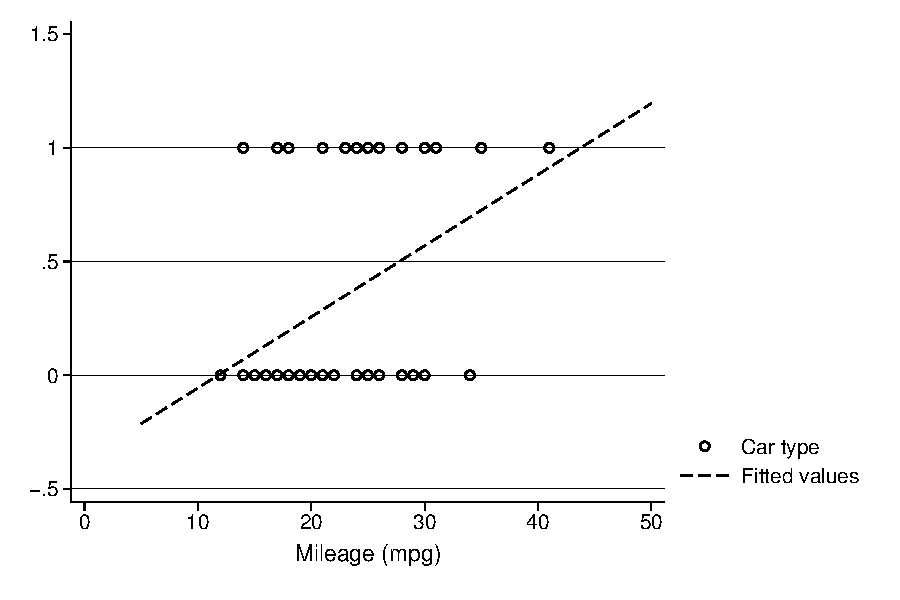
\includegraphics[width=\linewidth]{fig/mpl}
			\caption{Modelo de Probabilidad Lineal (MPL)}
			\label{img1}
		\end{minipage}
		\hfill
		\begin{minipage}{.48\linewidth}
			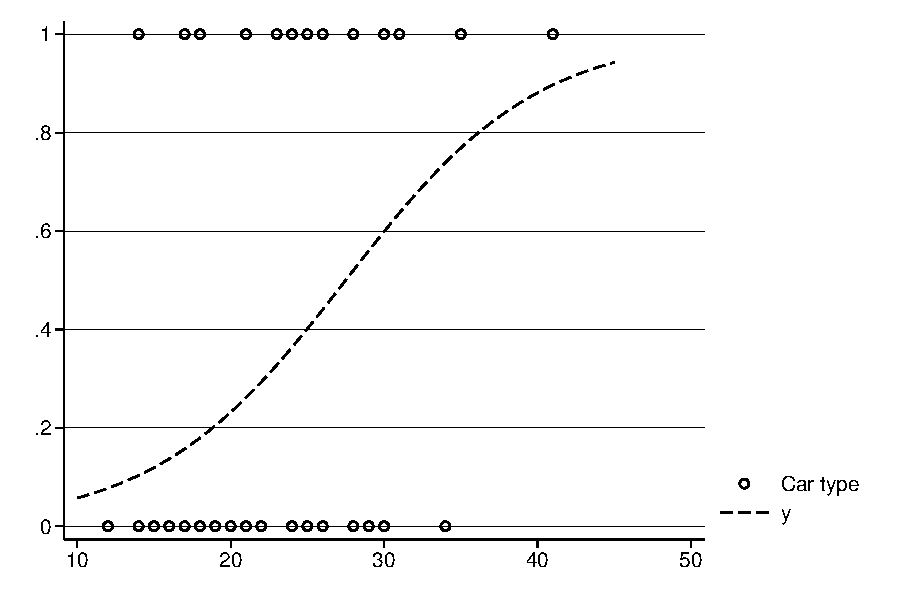
\includegraphics[width=\linewidth]{fig/mpnl}
			\caption{Modelo de Probabilidad No lineal}
			\label{img2}
		\end{minipage}
	\end{figure}
	
\end{frame}

\begin{frame}
	
	En teoría son varias las funciones no lineales que se
	pueden usar pero las mas populares son:
	\bigskip
	
	\begin{description}
		\item[Modelo Probit] $F(\omega)=\int_{-\infty}^{\omega}\frac{1}{\sqrt{2\pi}}e^{-t^2/2}dt$
		\item[Modelo Logit] $F(\omega)=L(\omega)=\frac{e^{\omega}}{1+e^{\omega}}$
	\end{description}
\end{frame}

\begin{frame}{Fundamento económico}
	Al menos dos justificaciones
	\begin{enumerate}
		\item Precio de reserva
		\item Modelo de utilidad aleatoria
	\end{enumerate}
\end{frame}


\subsubsection{Interpretación}

\begin{frame}{Efecto Marginal}
	
	El efecto marginal para la persona $i$ en la variable $k$, cuando
	la variable $x_k$ es continua se define como:
	
	\begin{eqnarray*}
		EM_{ik}=\frac{\partial Prob(Y_i=1)}{\partial x_k}=\frac{\partial F(X_i'\beta)}{\partial
			x_k}=\beta_k f(X_i'\beta)
	\end{eqnarray*}
	
	Mientras que cuando esta es dicotómica el efecto se define como:
	
	\begin{eqnarray*}
		EM_{ik}=F(X_i'\beta|x_k=1)-F(X_i'\beta|x_k=0)
	\end{eqnarray*}
\end{frame}

\begin{frame}{Comparación de Efectos Marginales}
	
	Una forma de comparar los resultados de los diferentes modelos es
	empleando efectos marginales:
	
	\begin{eqnarray}
		\frac{\partial}{\partial
			x_{ik}}x_i'\beta &=& \beta_k^{PL} \\
		\frac{\partial}{\partial x_{ik}}\Phi(x_i'\beta) &=& \phi(x_i'\beta)\cdot
		\beta_k^{Probit}\\
		\frac{\partial}{\partial x_{ik}}L(x_i'\beta) &=& \frac{e^{x_i'\beta}}{(1+e^{x_i'\beta})^2}\cdot
		\beta_k^{Logit}
	\end{eqnarray}
	
	Así, cuando $x_i'\beta=0$, se pueden tener ``equivalencias'' entre
	los distintos $\beta$s al igualar los efectos marginales de (1)
	con (2) y los efectos marginales de (1) y (3).
\end{frame}

\begin{frame}{Odds Ratios}
	
	En el caso de un logit del tipo:
	\begin{eqnarray}
		% \nonumber to remove numbering (before each equation)
		Pr[Y_j=1|X_j] &=& \frac{exp(\alpha_0+\beta_0 X_j)}{1+exp(\alpha_0+\beta_0 X_j)}
	\end{eqnarray}
	
	
	\textbf{Los odds} se definen como:
	
	\begin{eqnarray}
		Odds(X) &=& \frac{Pr[Y_j=1 | X_j]}{Pr[Y_j=0 | X_j]}=\frac{F(\alpha_0+\beta_0 X_j)}{1-F(\alpha_0+\beta_0
			X_j)}=exp(\alpha_0+\beta_0 X_j)
	\end{eqnarray}
	
	
	\textbf{Los odds ratios} es el ratio de dos odds para diferentes
	valores de $X_j$, digamos $X_j=x$ y $X_j=x+\Delta x$:
	
	\begin{eqnarray*}
		\frac{Odds(x+\Delta x)}{Odds(x)} &=& \frac{exp(\alpha+\beta x+\beta \Delta x)}{exp(\alpha+\beta
			x)}=exp(\beta \Delta x)
	\end{eqnarray*}
	
	%Tomando logaritmos...
\end{frame}


\subsection{Estimación}

\begin{frame}[fragile]
	\frametitle{Estimación}
	\begin{itemize}
		\item Se emplea MV
		
		\item Sea una muestra $y_1, y_2..., y_n$ cuya probabilidad de
		ocurrir es $P(muestra)$
		
		\item $P(muestra)=P(y_1)*P(y_2)*P(y_2)...*P(y_n)$, si cada
		$y_i$  es independiente
		
		\item Donde $P(y_i)=1-F(X_i\beta)$  si $y1=1$  o $P(y_i)=F(X_i\beta)$  si
		$y_i=0$
		
		\item La función de verosimilitud:
		\begin{eqnarray*}
			L &=& \Pi_{y_i=1}[1-F(-X_i\beta)]*\Pi_{y_i=0}F(-X_i\beta)
		\end{eqnarray*}
		
		\item Los $\beta$s los encontramos maximizando esta función
		(matemáticamente es un proceso iterativo, se empieza con un
		grupo de $\beta$s y se va iterando hasta alcanzar los $\beta$s óptimos)
	\end{itemize}
\end{frame}

%\subsection{Efectos Marginales}
%
%\begin{frame}[fragile]
%  \frametitle{Efectos Marginales}
%\begin{itemize}
%    \item La interpretación no es la misma que en un modelo lineal
%    
%    \item El impacto del las variables independientes (efecto marginal)
%     es diferente dependiendo del punto en el cual se calcula el impacto:
%    \begin{eqnarray*}
%      \frac{\partial F(X_i\beta)}{\partial x_{ik}} &=&
%      f(X_i\beta)\beta_k
%    \end{eqnarray*}
%    
%    \item Donde $f$ es la función de densidad de probabilidad (p.d.f)
%    
%    \item Puntos cercanos a la media tienen un impacto mucho mayor comparados con puntos en las `colas' de la distribución.
%\end{itemize}
%\end{frame}

\subsubsection{Logit nulo, ingenuo o baseline}

\begin{frame}[fragile]
	\frametitle{Modelo ingenuo}
	
	Estime el modelo logit ingenuo sabiendo que:
	\bigskip
	
	\begin{tabular}{c}
		% after \\: \hline or \cline{col1-col2} \cline{col3-col4} ...
		\hline
		Y \\
		\hline
		1 \\
		0 \\
		0 \\
		\hline
	\end{tabular}
\end{frame}

\subsubsection{Generalización}

\begin{frame}[fragile]
	\frametitle{Generalización}
	
	Sea $(y_i,x_i)$ con $i=1,...,n$, una muestra $iid$ $Y_i$ tiene una
	distribución de Bernoulli con $p_i=Pr(y_i=1)$ con lo cual la
	función de verosimilitud será:
	
	
	\begin{eqnarray*}
		L(\beta) &=& \prod_{y_i=1}p_i \prod_{y_i=0}(1-p_i)=\prod_{i=1}^n p_i^{y_i}(1-p_i)^{1-y_i}
	\end{eqnarray*}
	
	
	
	y su logaritmo:
	
	\begin{eqnarray*}
		l(\beta) &=& \sum_{i=1}^n [y_i (ln p_i)+(1-y_i)ln(1-p_i)] \\
		&=& \sum_{i=1}^n [y_i ln F(x_i'\beta)+(1-y_i)ln(1-F(x_i'\beta))]
	\end{eqnarray*}
	
\end{frame}

\begin{frame}[fragile]
	\frametitle{Generalización}
	
	Siendo las condiciones de primer orden:
	
	\begin{eqnarray*}
		\sum_{i=1}^n\frac{(y_i-F_i)f_i}{F_i(1-F_i)}x_{ki}&=&0
	\end{eqnarray*}
	
	con $k=1,...,K$; $F_i\equiv F(x_i'\beta)$ y $f_i\equiv
	f(x_i'\beta)$
	\smallskip
	
	
	
	En el caso particular de un logit
	$(F(x)=\frac{exp(x)}{1+exp(x)})$ la expresión se reduce a:
	
	\begin{eqnarray*}
		\frac{\partial \ln L}{\partial \theta }&=&\sum_{i=1}^{n}(y_{i}-F_i)\mathbf{x}%
		_{i}=\mathbf{0}
	\end{eqnarray*}
\end{frame}

\subsection{Curvas ROC}

\begin{frame}[fragile]
	\frametitle{Curvas ROC}
	\begin{itemize}
		\item  ¿Cómo predecir la ocurrencia de un evento a partir de la estimación de un modelo tipo probit
		o logit? (buen o mal pagador)
		\item Los modelos permiten calcular las probabilidades de
		ocurrencia, típicamente se asume que si la probabilidad predicha
		es superior a 0.5, entonces se asume que el evento ocurrirá.
		\item Reconocer que existen dos tipos de errores que se cometen cuando se
		hace la predicción discreta es la motivación de la estrategia
		ROC.
		\item El porcentaje de unos clasificados incorrectamente y el porcentaje de ceros clasificados
		incorrectamente se conocen como sensitividad y especificidad,
		respectivamente.
	\end{itemize}
\end{frame}

\begin{frame}[fragile]
	\frametitle{Curvas ROC}
	\begin{table}
		\centering
		\begin{tabular}{cccc}
			\hline \hline
			& \multicolumn{ 2}{c}{Verdadero} &            \\
			
			Clasificado &          D=1 &         D=0 &      Total \\
			\hline
			+ &          a &          c &        a+c \\
			
			- &          b &          d &        b+d \\
			\hline
			Total &        a+b &        c+d &    a+b+c+d \\
			\hline
		\end{tabular}
		\caption{Classified es $+$ si Pr(D) predicha $>=$ umbral}
	\end{table}
	
	Donde ``Verdadero'' hace referencia a lo efectivamente observado
	(lo verdadero), D=1 y ~D=0 y ``Classified'' es lo estimado
	probabilísticamente.
\end{frame}

\begin{frame}[fragile]
	\frametitle{Curvas ROC}
	Si la probabilidad de ocurrencia es mayor a un determinado umbral
	(por ejemplo $0.5$), entonces se clasifica como cierto la
	ocurrencia (+). A partir de lo predicho y lo efectivamente
	observado se pueden construir los siguientes indicadores:
	
	
	\begin{enumerate}
		\item \texttt{Sensitibidad:} Porcentaje de unos clasificados
		correctamente: $\frac{a}{a+b}$
		
		\item \texttt{Especificidad:} Porcentaje de ceros clasificados
		correctamente: $\frac{d}{c+d}$
		
		\item \texttt{Correctamente clasificados:} Total de correctamente clasificados: $\frac{a+d}{a+b+c+d}$
	\end{enumerate}
\end{frame}

\begin{frame}[fragile]
	\frametitle{Curvas ROC. Presentación gráfica}
	\begin{figure}
		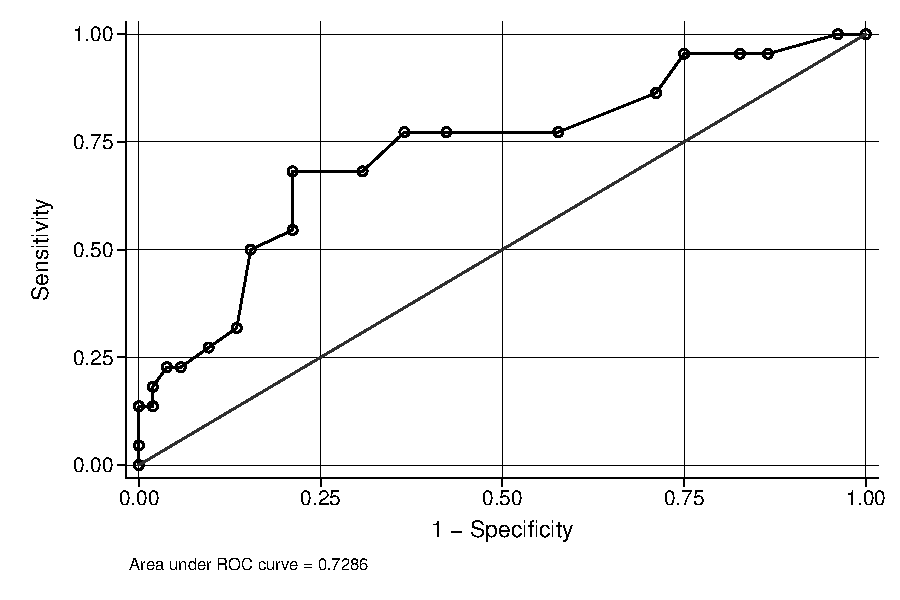
\includegraphics[scale=.6]{fig/lroc}
		\caption{Curva ROC.}
	\end{figure}
\end{frame}

\begin{frame}[fragile]
	\frametitle{Curvas ROC. Selección de modelos}
	
\end{frame}



\subsubsection{Evaluación del modelo}

\begin{frame}[fragile]
	\frametitle{Bondad de ajuste}
	\begin{itemize}
		\item Pseudo-R2 que compara la función de verosimilitud maximizada por nuestros betas con una función
		donde todos los betas son cero y solo hay una constante (modelo ingenuo)
		
		\item Formalmente: Test LR  (Likelihood ratio)
		
	\end{itemize}
\end{frame}